\documentclass[a4,landscaep]{article}
\usepackage{tikz}
\begin{document}

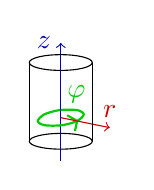
\begin{tikzpicture}

%koordinaatisto
\draw[blue!75!black](0,-.25,0)--(0,.30,0);
\draw[green!80!black, thick] plot [smooth cycle] coordinates{(.25,.30,.11) (.11,.30,.25) (-.11,.30,.25) (-.25,.30,.11) (-.25,.30,-.11)(-.11,.30,-.25) (.11,.30,-.25) (.25,.30,-.11)};
\draw[green!80!black, thick] (.1,.35,.05) -- (.25,.30,.11) -- (.2,.15,.05);
\node at (.2,.6,0) {$\textcolor{green!80!black}\varphi$};
\draw[blue!75!black, ->](0,.30,0)--(0,1.25,0) node[left] {$\textcolor{blue!75!black}z$};
\draw[red!80!black, ->](0,.30,0) --(.75,.30,.33) node[above] {$\textcolor{red!80!black}r$};

%sylinteri
\draw (0,1) coordinate (top) circle[x radius=.4, y radius = 0.1];
\draw (.4, 1) -- (.4, 0);
\draw (-.4, 1) -- (-.4, 0);
\draw (0,0) coordinate (bottom) circle[x radius=.4, y radius = 0.1];

\end{tikzpicture}

\end{document}